\clearpage

\section{Konkurrentanalyse}

Målet med konkurrentanalysen er å finne inspirasjon til nettstedet vi skal utvikle ved å se på allerede eksisterende løsninger. Hvem er oppdragsgiver sine konkurrenter? Hvordan type løsning har disse valgt? Hvilke styrker og svakheter har løsningene? Analysen er først og fremst gjort av gruppen med vekt på å se det fra en vanlig bruker sitt perspektiv, men noen tekniske faktorer har også blitt vurdert.

\subsection{Teknisk analyse}
For å vurdere de tekniske faktorene har vi brukt Google Lighthouse til å sjekke hvor raskt nettstedene lastes inn, beste praksis og SEO. I tillegg ble WAVE \footnote{Web Accessibility Evulation Tool. http://wave.webaim.org/} brukt til å sjekke om nettstedene følger kravene for loven om universell utforming og tilgjengelighet.

\subsection{Konkurrentene}
Sirkus Media har mange konkurrenter, deriblant alle firmaer som driver mediebyråvirksomhet. Etter samtale med Hans Christian Hymer \footnote{Samtale med oppdragsgiver (16.01.2019)} fikk vi oppgitt 3 bedrifter som blir ansett som Sirkus Media sine største konkurrenter. Det er følgelig disse konkurrentene vi har valgt å analysere.

\subsection{TACTIC™ Real-Time Marketing}
Nettstedet til TACTIC™ Real-Time Marketing ligger på følgende domene; https://tacticrealtime.com. Se figur \ref{fig:competitors-tacticrealtime.com} for bilde av nettstedet.

\subsubsection{Førsteinntrykk}
Førsteinntrykket er at nettstedet fremstår ryddig og profesjonelt. Det første som møter deg er et stort bakgrunnsbilde. Bilde dekker hele skjermen og har en tittel og en underoverskrift. Headeren består også av en knapp der du kan trykke på \q{Request a demo}. Helt øverst på forsiden er logoen til Tactic og en meny. Til høyre er det en knapp som gir deg muligheten til å se på en video. 

\begin{figure}[H]
    \centering
    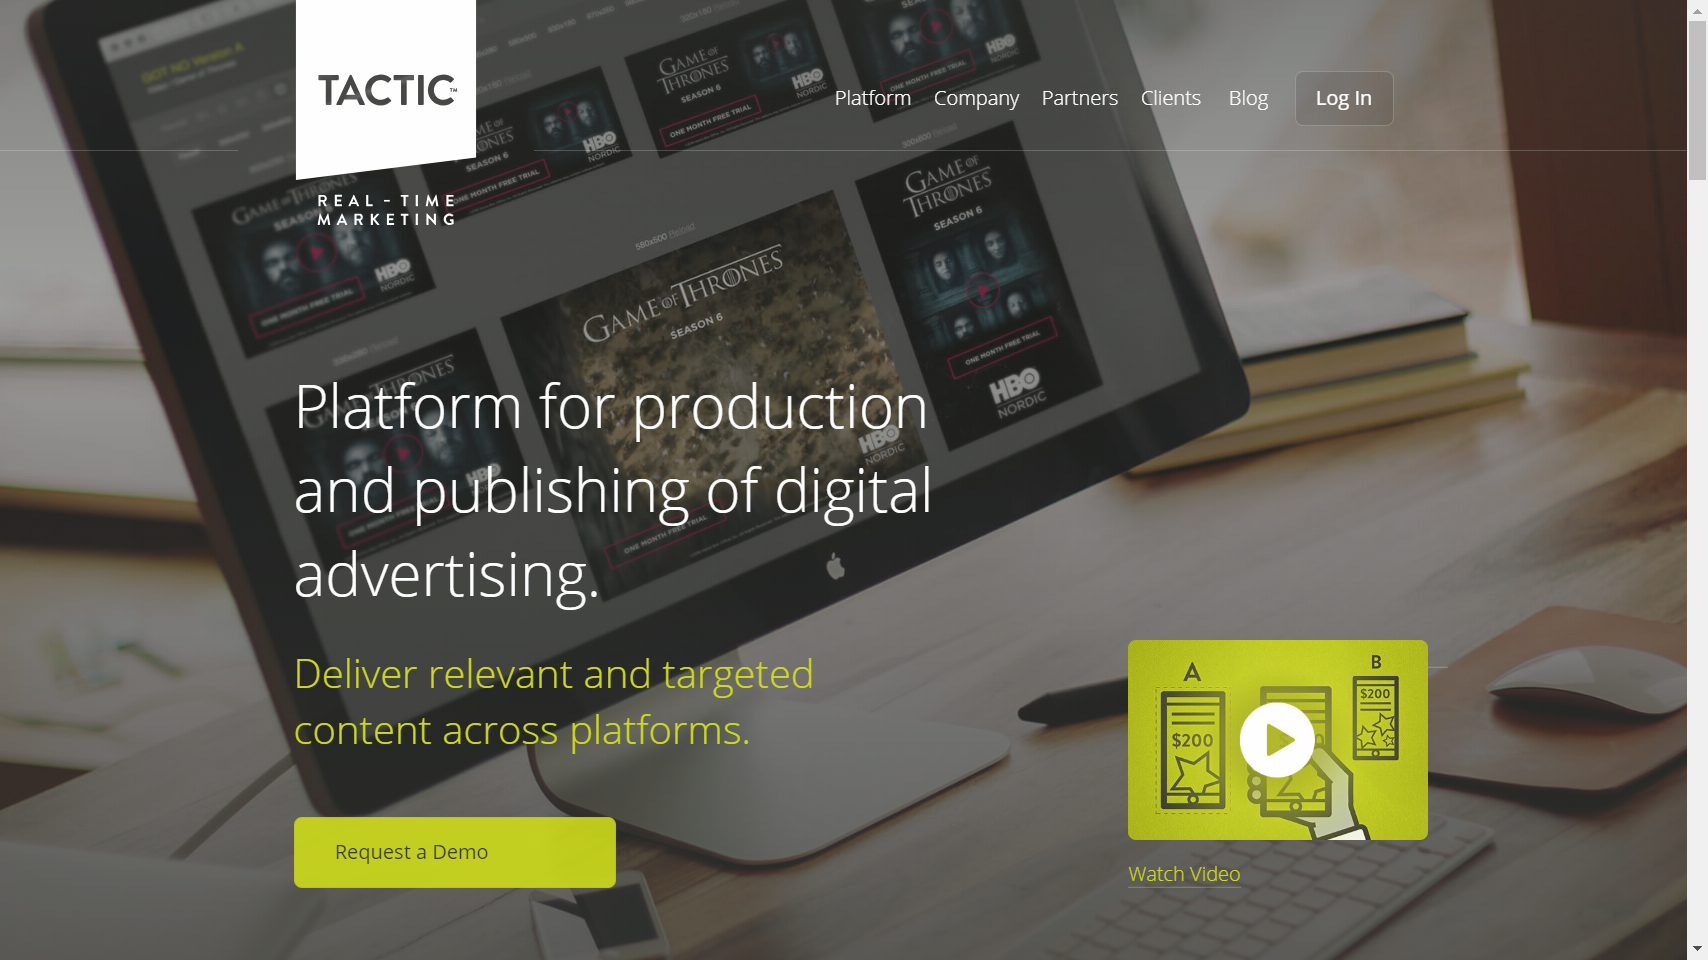
\includegraphics[width=\textwidth]{line/tacticrealtime_com_(1366x768).png}
    \caption{tacticrealtime.com}
    \label{fig:competitors-tacticrealtime.com}
\end{figure}

\subsubsection{Forside og undersider}

Forsiden består av bakgrunnsbilde som inneholder logo, meny, overskrifter og en video.  
Deretter kommer det en beskrivende tekst om firmaet, informasjon om plattformen, logo av ledende  Ad-servers og DSP's, partnerprogram og utvalgte kunder. Siden avsluttes med en \q{Contact us}-seksjon.

Nettstedet består også av følgende undersider:
\begin{itemize}
\item Platform
\item Company
\item Partners
\item Clients
\item Blog
\end{itemize}

\subsubsection{Teknisk analyse}

\begin{figure}[H]
    \begin{center}
        \subfigure[Google lighthouse]{
            \label{fig:competitors-lighthouse-summary-tacticrealtime.com}
            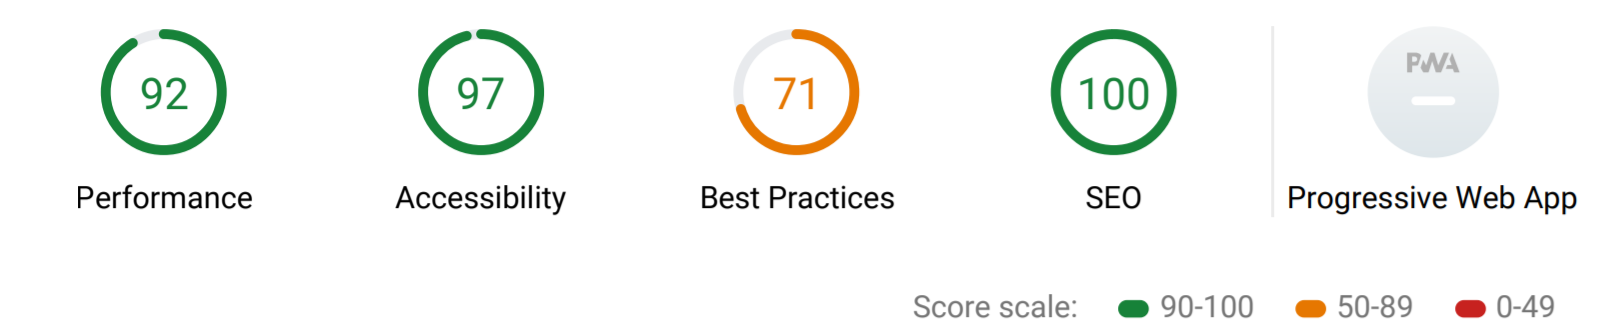
\includegraphics[width=0.7\textwidth]{line/tacticrealtime_com-lighthouse.png}
        }
        \rulesepv
        \subfigure[WAVE]{
            \label{fig:competitors-wave-summary-tacticrealtime.com}
            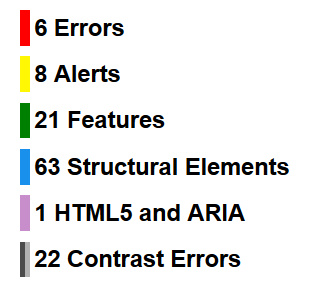
\includegraphics[width=0.2\textwidth]{line/tacticrealtime_com-wave.png}
        }
        
        \label{fig:competitors-tech_analysis-tacticrealtime.com}
        \caption{Resultat fra teknisk analyse av tacticrealtime.com}
    \end{center}
\end{figure}

Etter å ha gjennomført testen til Google Lighthouse, viste det seg at TACTIC var den desidert beste på alle punkter av de 3 konkurrentene. Restultatene fra Google Lighthouse kan man se i figur \ref{fig:competitors-lighthouse-summary-tacticrealtime.com}. Bedriften gjør relativt få feil med tanke på ytelse. Feilene som gjelder \q{Eliminate render-blocking resources}\footnote{Hva vil dette si?} og \q{Serve static assets with an efficient cache policy}\footnote{Hva vil dette si?} burde rettes opp. Vi kan se at siden lastet inn på 2,7 sekunder. Fikser man de overnevnte feilene, vil man kunne mer enn halvere innlastningstiden i følge rapporten.

Når det kommer til \q{Best Pracices}, så er det et par forbedringer TACTIC burde gjort. De burde benytte HTTP2, i stedet for HTTP \footnote{HTTP2 er bakoverkompatibel, så ingen grunn til å ikke bruke det. Samt at det pleier å være 1 linje med kode for å skru på for de fleste web-servere.}. Det linkes også til et JavaScript-bibliotek med kjente sikkerhetshull. Dette burde man på ingen måte gjøre.

På SEO-delen av testen fikk TACTIC 100 av 100 poeng og det er derfor ingenting å påpeke her.

Full rapport for Google Lighthouse kan leses i vedlegg X1.

Figur \ref{fig:competitors-wave-summary-tacticrealtime.com} viser resultatene fra WAVE. Fra resultatene ser man at Tactic fikk 6 feilmeldinger når det kommer til universell utforming. I tillegg har nettsiden deres 22 kontrastfeil. 

\subsubsection{Styrker}
En stor fordel er at nettstedet gir et bra førsteinntrykket. Dette fordi nettstedet fremstår som profesjonelt. Førsteinntrykket er dermed med på å styrke brukerens inntrykk av bedriften. Nettstedet har også god oppbygning og struktur. Løsningen har også en sterk profil, hvor det er ganske tydelig at det er grønn som er primærfargen til selskapet.

\subsubsection{Svakheter}
Noe som kan være en svakhet er at hele nettstedet er på engelsk og i tillegg er på et .com-domene. Disse to faktorene kan forvirre brukerne. En av grunnen til dette er at det er vanskelig å skjønne at dette er et firma som er lokalisert i Oslo. En annen svakhet er at det er lite luft rundt noen elementer, som fører til at nettstedet fremstår som kompakt og mer rotete. Det er heller ikke samme mengde luft over og under elementene. Dette er også med på å trekke ned helhetsinntrykket. Det er heller ikke så lett å bevege seg rundt på nettstedet ved hjelp av tastaturet ettersom TACTIC har fjernet all visuell indikasjon for fokus. Dette gjør at nettsiden ikke oppfyller noe som er et krav i loven om universell utforming og tilgjengelighet. I tillegg får nettstedet mange kontrastfeil, som også bryter lovkravet om universell utforming.

\subsection{Marketer Technologies AS}
Nettstedet til Marketer Technologies AS ligger på følgende domene;
https://marketer.tech/. Se figur \ref{fig:competitors-marketer.tech} for bilde av nettstedet.

\subsubsection{Førsteinntrykk}
Førsteinntrykket av nettstedet er positivt, fordi den fremstår som ryddig og profesjonell. Det første som møter deg er headeren\footnote{Hodet til nettstedet} til nettstedet, som inneholder logoen til firmaet og en meny. Under menyen er en tittel, en underoverskrift og to lenker. Headeren inneholder også et ikon for chat. Det at kunder enkelt kan ta kontakt med firmaet kan virke betryggende, og kan være med å øke troverdigheten til bedriften.

\begin{figure}[H]
    \centering
    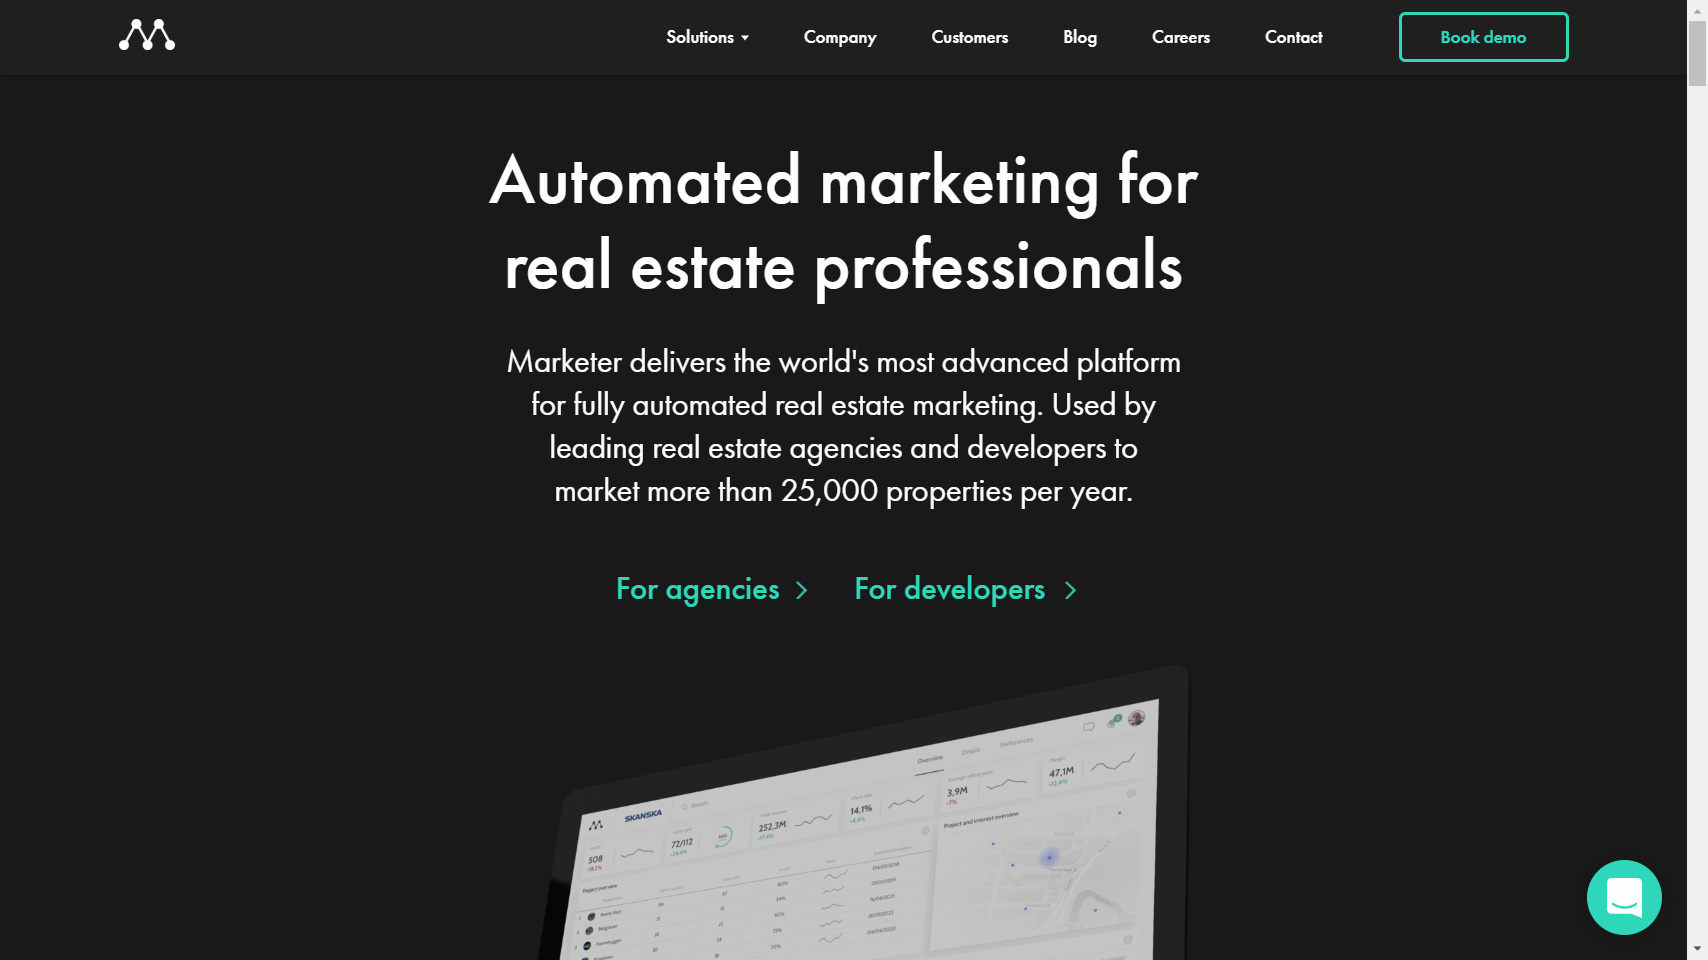
\includegraphics[width=\textwidth]{line/marketer_tech_(1366x768).png}
    \caption{marketer.tech}
    \label{fig:competitors-marketer.tech}
\end{figure}

\subsubsection{Forside og undersider}

Forsiden, i tillegg til headeren, består av logo til noen utvalgre kunder, prosessen til Marketer, animasjoner, resultater fra tidligere prosjekter og en presentasjon av deres løsninger. Helt nederst på siden kommer bunnfeltet, der organisasjonsnummeret, kontaktinformasjon og adresse blir presentert.

Nettstedet består også av følgende undersider:
\begin{itemize}
\item Solutions
\item Company
\item Customers
\item Blog
\item Careers 
\item Contact
\item Book demo
\end{itemize}

\subsubsection{Teknisk analyse}
\begin{figure}[H]
    \begin{center}
        \subfigure[Google lighthouse]{
            \label{fig:competitors-lighthouse-summary-marketer.tech}
            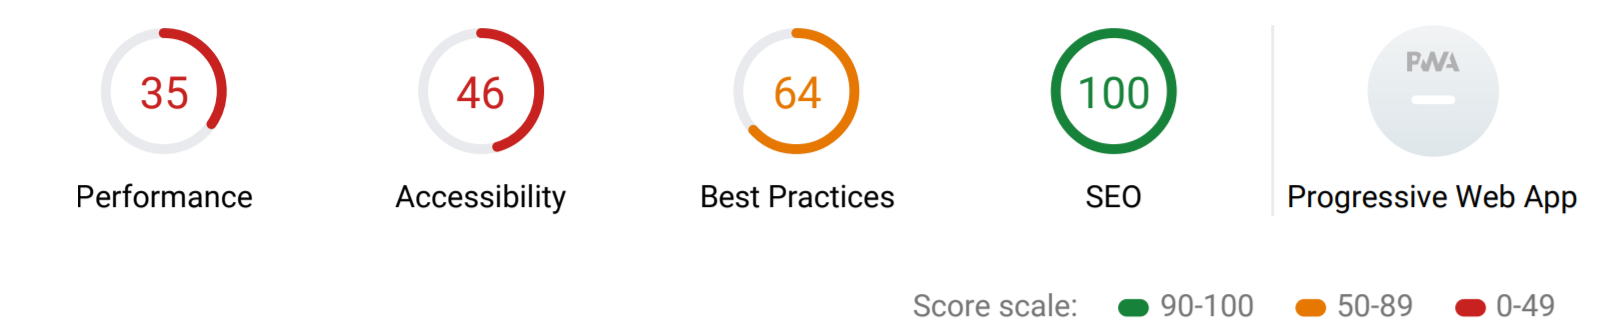
\includegraphics[width=0.7\textwidth]{line/marketer_tech-lighthouse.png}
        }
        \rulesepv
        \subfigure[WAVE]{
            \label{fig:competitors-wave-summary-marketer.tech}
            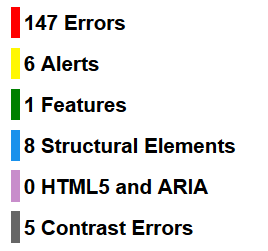
\includegraphics[width=0.2\textwidth]{line/marketer_tech-wave.png}
        }
        
        \label{fig:competitors-tech_analysis-marketer.tech}
        \caption{Resultat for teknisk analyse av marketer.tech}
    \end{center}
\end{figure}

Figur \ref{fig:competitors-lighthouse-summary-marketer.tech} viser resultatene fra testen gjort med Google Lighthouse. Her kom Marketer dårligst ut. Testen påpeker flere feil på punkter vedrørende ytelse, tilgjengelighet og beste praksiser. Det tar Google 5,3 sekunder å laste inn nettstedet, noe som er relativt tregt, men det er raskere enn Inviso.no. Selv om Marketer sin side laster inn raskere, så får den en dårligere poengsum på ytelse. Dette fordi det tar hele 15,2 sekunder før siden blir beregnet som interaktiv \footnote{\q{Time to Interactive} i Google Lightouse rapporten}. Marketer burde ta samme grep som TACTIC, i tillegg til å fjerne ubrukt CSS, servere skalerte bilder og vurdere å redusere antall animasjoner.
Full rapport for Google Lighthouse kan leses i vedlegg X2.

Figur \ref{fig:competitors-wave-summary-marketer.tech} viser WAVE-resultatene. Her kommer det frem at løsningen har 5 kontrastfeil og hele 147 feil når det kommer til universell utforming og tilgjengelighet. 135 av disse feilmeldingene er manglende bruk av alt-tekster.

\subsubsection{Styrker}
En av styrkene er at nettstedet gir et bra førsteinntrykk. Det er også et nettsted som skiller seg ut og er gjennomført. En annen styrke er at løsningen inneholder chat, der kunder enkelt kan ta kontakt. Profilen er også klar og tydelig, og det er åpenbart at bedriften har sort som primærfarge og turkis som aksentfarge.

\subsubsection{Svakheter}
En ulempe er at nettstedet består av flere store filer, som fører til at nettstedet oppleves som tregt. En annen svakhet er at løsningen får mange feil når det kjøres tester på universell utforming og tilgjengelighet. Det er i tillegg vanskelig å navigere seg rundt på nettstedet ved hjelp av kun tastatur.


\subsection{Inviso AS}
Nettstedet til Inviso AS ligger på følgende domene;
https://www.inviso.no/. Se figur \ref{fig:competitors-inviso.no} for bilde av nettstedet.

\subsubsection{Førsteinntrykk}
Førsteinntrykket av nettstedet er at den fremstår som rotete. Hovedgrunnen til dette er at det er mange elementer og mye som skjer i headeren. Logoen og noe av teksten på bakgrunnsbilde er også vanskelig å se på grunn av det dårlige kontrastforholdet. 

\begin{figure}[H]
    \centering
    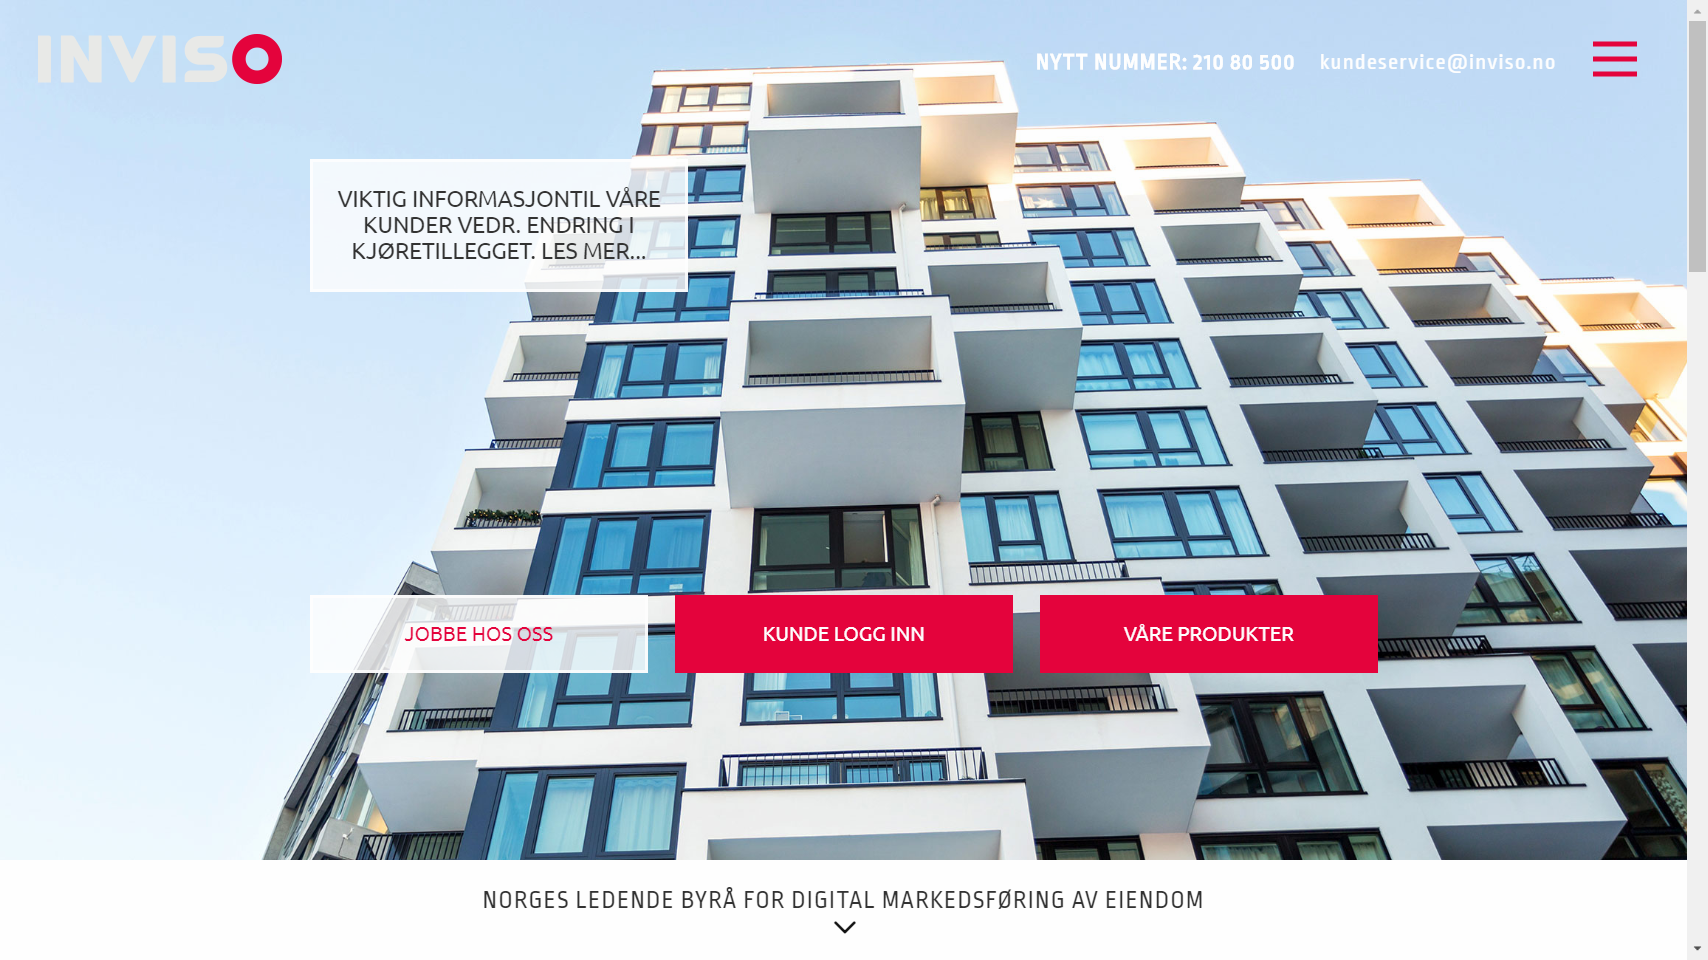
\includegraphics[width=\textwidth]{line/inviso_no_(1366x768).png}
    \caption{inviso.no}
    \label{fig:competitors-inviso.no}
\end{figure}

\subsubsection{Forside og undersider}
I tillegg til headeren består forsiden av \q{Om oss}-tekst, deres tjenester og utvalgte kunder. 

Nettstedet består også av følgende undersider:
\begin{itemize}
\item Inviso
\item Våre produkter
\item Kontakt
\item Galleri
\item Verktøy
\item Nyheter
\end{itemize}


\subsubsection{Teknisk analyse}

\begin{figure}[H]
    \begin{center}
        \subfigure[Google lighthouse]{
            \label{fig:competitors-lighthouse-summary-inviso.no}
            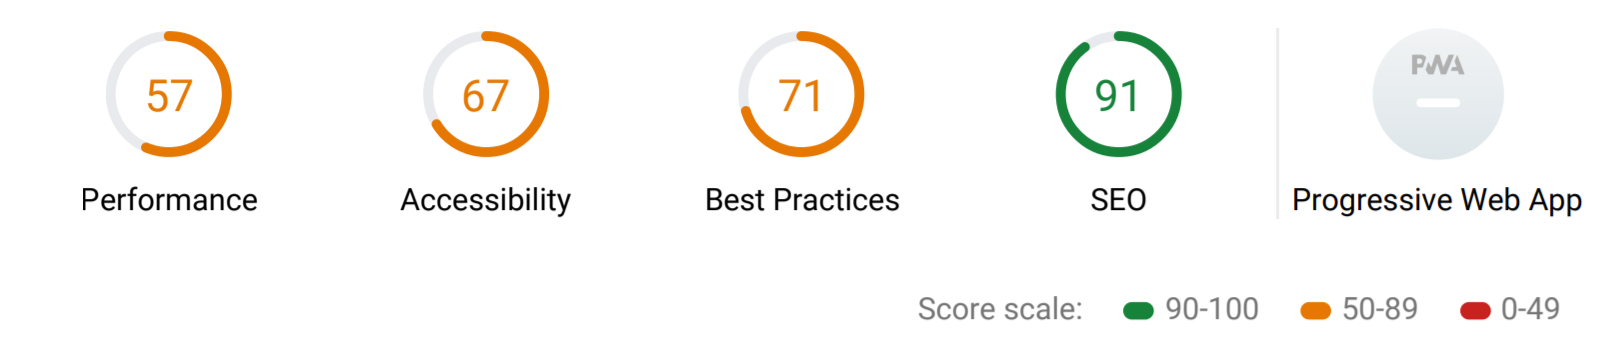
\includegraphics[width=0.7\textwidth]{line/inviso_no-lighthouse.png}
        }
        \rulesepv
        \subfigure[WAVE]{
            \label{fig:competitors-wave-summary-inviso.no}
            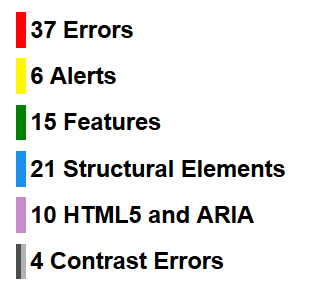
\includegraphics[width=0.2\textwidth]{line/inviso_no-wave.png}
        }
        
        \label{fig:competitors-tech_analysis-inviso.no}
        \caption{Resultat for teknisk analyse av inviso.no}
    \end{center}
\end{figure}

Figur \ref{fig:competitors-lighthouse-summary-inviso.no} viser resultatene fra testen gjort av Google Lighthouse. Her havnet Inviso midt på treet og kom dermed på andre plass av de tre konkurrentene. Bedriften får en helt grei poengsum i gjennomsnitt. Når det kommer til ytelse, bør de ta samme grep som både TACTIC og Marketer. Hovedproblemet her er at bildene serveres i en lite egnet filtype, og kan enkelt løse ved å velge en filtype som er mer egnet. Ved å fikse dette kan de hente inn hele 4,2 sekunder av den totale innlastningstiden på 6,7 sekunder.

På test delen vedrørende tilgjengelighet kommer det frem av Inviso burde forbedre kontrastforhold på deler av siden sin.

Ingenting spesielt å påpeke ved SEO, men Inviso burde absolutt ta en titt på hvilke JavaScript-biblioteker de bruker, ettersom Google kan melde om hele 5 kjente sikkerhetshull er tilgjengelig på siden. Full rapport for Google Lighthouse kan leses i vedlegg X3.

Ved å kjøre test via WAVE oppgir resultatet at nettstedet har 4 kontrastfeil. Nettstedet får også 37 feilmeldinger når det gjelder universell utforming. Figur \ref{fig:competitors-wave-summary-inviso.no} viser resultatene fra WAVE-testen.

\subsubsection{Styrker} 
En av styrkene er at nettstedet har en bra profil. Det er lett å skjønne at rød er primærfargen til Inviso. En annen positiv side er at det tekstlige innholdet på siden er godt skrevet og får bedriften til å fremstå profesjonelt.

\subsubsection{Svakheter}
En svakhet er at det er for mye informasjon i headeren. Dette kan bidra til at førsteinntrykket blir dratt ned. En annen stor svakhet er at nettstedet får mange feil når man kjører tester når det gjelder universell utforming og tilgjengelighet. Det faktum at nettsiden har en mobil-meny på fullversjon av siden, trekker også ned fordi dette gjør brukeropplevelsen dårligere.

\subsection{Konklusjon}
Felles for alle 3 konkurrentene er at ingen av de følger loven om universell utforming og tilgjengelighet. Universell utforming er lovpålagt i Norge \footnote{\url{https://lovdata.no/dokument/SF/forskrift/2013-06-21-732}}, og vår løsning kommer derfor til å følge disse kravene. 

En annen faktor konkurrentene har til felles er at de presenterer sine kunder og/eller partnere. Dette bør også Sirkus Media gjøre. Presentasjon av kundeforhold med kjente firmaer er tillitsvekkende og kan skape bedre troverdighet blant brukerne. \footnote{Kilde?}

Figur \ref{fig:competitors-mobile} viser at alle konkurrentene har gått for samme løsning når det kommer til design på mobil. Alle har bedriftens logo oppe til venstre og et meny ikon til høyre. Undersøkelser \footnote{Kilde: Luke Wroblewski, en internasjonalt anerkjent brukeropplevelsesdesigner \url{https://www.lukew.com/ff/entry.asp?1945}} viser at dette er langt fra den mest optimale løsningen. Planen er derfor at vår løsning skal ha en annen struktur.

Konkurrentene har gode løsninger, men også en del svakheter som har blitt påpekt i denne analysen. Konkurrentanalysen har vært nyttig fordi den både har ført til at gruppen har fått inspirasjon til deler av den løsningen som skal utvikles og samtidig gitt en pekepinn på hva som bør gjøres annerledes.

Studentgruppen har satt som mål å få minst like bra score på testen til Google Lighthouse, som gjennomsnittsscoren til de utvalgte konkurrentene.

\begin{figure}[bh]
    \begin{center}
        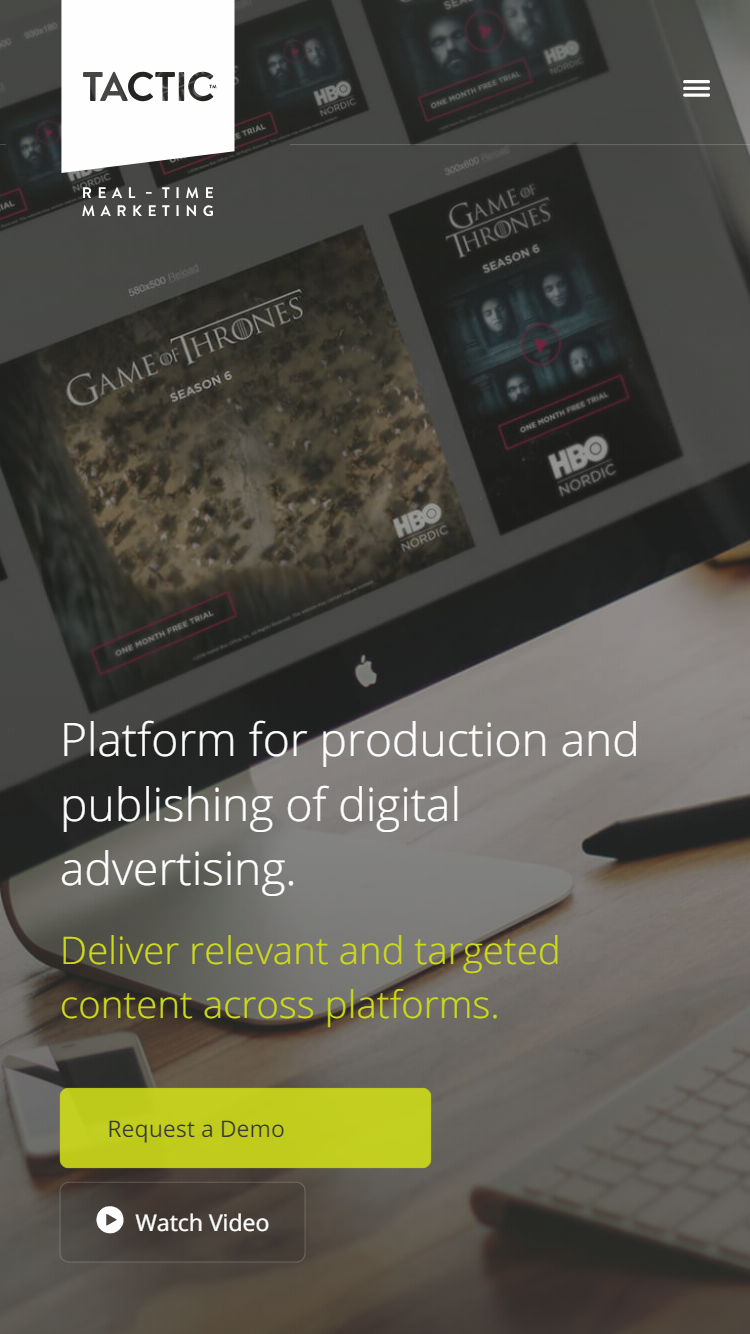
\includegraphics[width=0.3\textwidth]{line/tacticrealtime_com_(iPhone_6_7_8).png}
        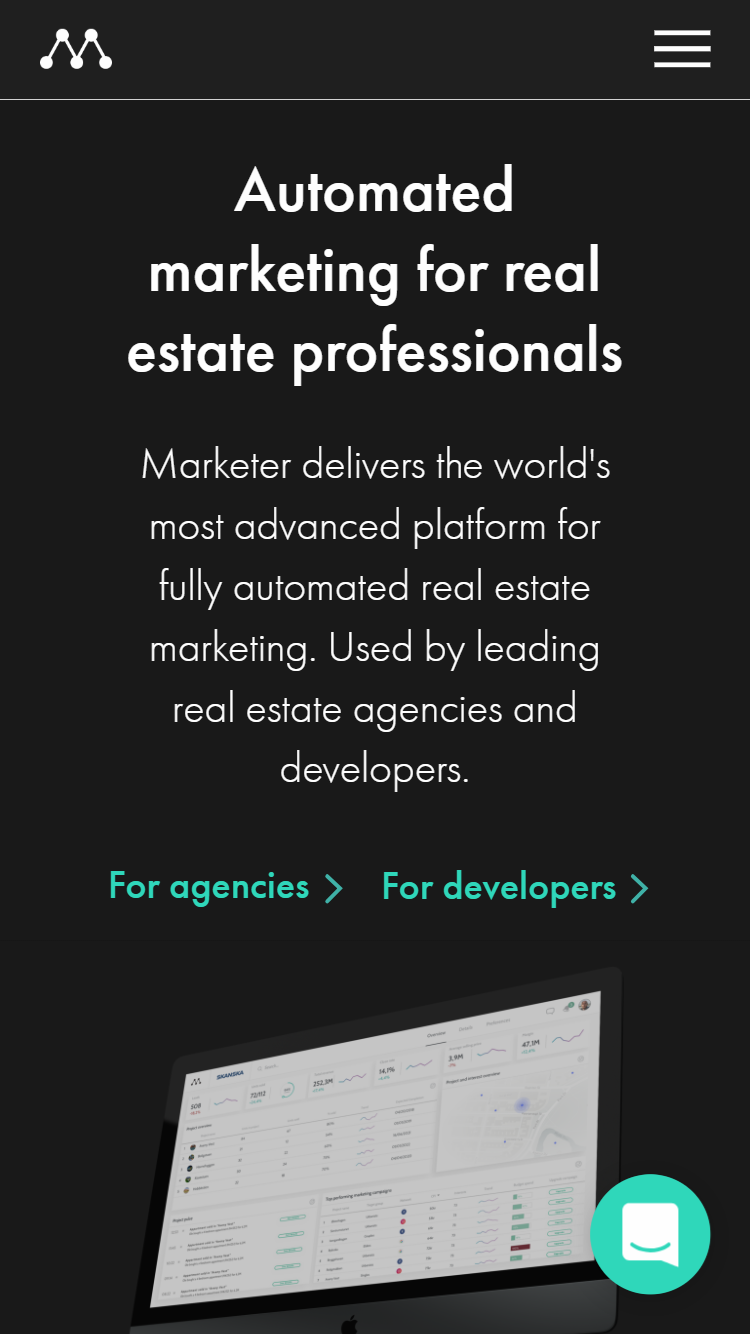
\includegraphics[width=0.3\textwidth]{line/marketer_tech_(iPhone_6_7_8).png}
        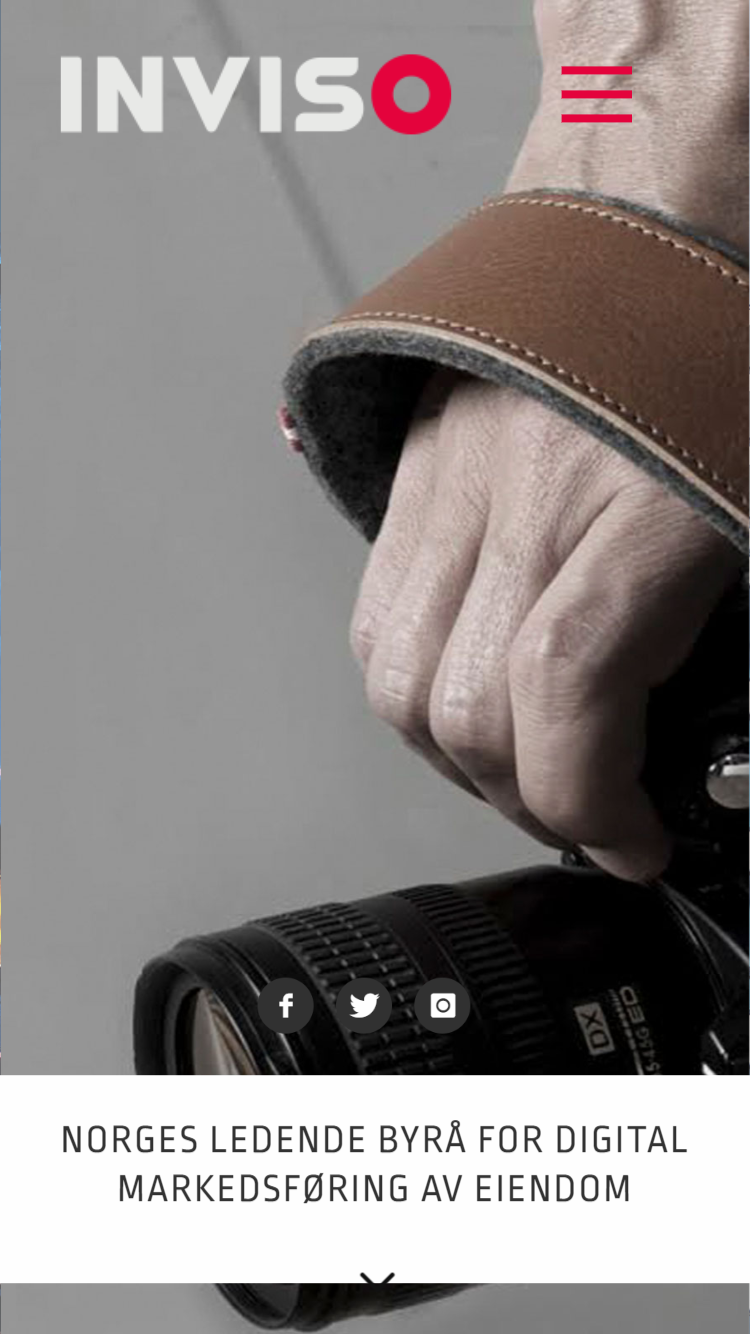
\includegraphics[width=0.3\textwidth]{line/inviso_no_(iPhone_6_7_8).png}
        \caption{Alle nettstedene er mobiltilpasset}
        \label{fig:competitors-mobile}
    \end{center}
\end{figure}

\section{Planlegging av struktur og innhold}

Struktur og innhold burde være som følgende: 

\textbf{Forside} Tanken er at hele nettstedet i hovedsak skal bestå av en lang forside. Fordi dette ikke er beste praksis for søkemotoroptimalisering vil vi forbedre SEO ved å lenke til nye sider som er mer detaljert. Høyt oppe på siden skal det være et kontaktskjema. Telefonnummeret til bedriften skal også være lett tilgjengelig. I tillegg skal forsiden bestå av en beskrivelse av bedriften, presentasjon av hva de tilbyr, steg for steg om prosessessen med animasjoner og omtale og logo fra eksisterende kunder. Videre skal nettstedet også ha et kart som er integrert med Google Maps, som viser lokasjonen til bedriften. Nederst på nettstedet skal det være organisasjonsnummer, link til personvern og logg inn.

\textbf{Meny} Nettstedets meny skal være tilgjengelig uavhengig av hvilken side brukeren står på. Her skal alltid forside, om oss og kontakt oss være tilgjengelig. 

\textbf{Om oss} Det vil også bli opprettet en egen \q{Om oss}-side som man kommer til ved å trykke \q{Les mer} på forsiden. Denne siden inneholder en mer detaljert presentasjon av Sirkus Media og deres historie.

\textbf{Kontakt oss} Nettstedet vil i tillegg til kontaktskjema på forsiden, bestå av en egen side med kontaktinformasjon. Her presenteres også relevant informasjon som bedriftens adresse, e-post, mobilnummer og kart. Vi lager en dedikert side for kontaktinformasjon fordi det er positivt med tanke på søkemotoroptimalisering. For eksempel: Hvis en bruker søker på Google etter Sirkus Media og det ikke er en egen side for kontakt oss, vil brukeren kun få treff på forsiden og undersidene med andre urelevante temaer. Siden brukeren ønsker å kontakt Sirkus Media,  hadde det vært mer brukervennlig å ha en link til kontakt siden i Google.

\textbf{Logg inn} Egen side der de ansatte kan logge inn for å komme til brukergrensesnittet for oppdatering og endring av innhold.

\textbf{Administrasjonsside}  På administrasjonssiden kan de ansatte endre og legge til innhold gjennom et brukergrensesnitt.

\textbf{Informasjon om personvern og informasjonskapsler} Personvernssiden skal inneholde en personvernserklæring. Denner forteller hvordan Sirkus Media samler inn og bruker personopplysninger. Målet er å gi brukerne overordnet informasjon om deres behandling av personopplysninger. I tillegg skal den fortelle brukeren hvilke informasjonskapsler som blir brukt på nettstedet.

\textbf{Annet} Alle sidene skal ha tilgang til en chat, der man kan ta direkte kontakt med oppdragsgiver.

\section{Definering av CMS}



\clearpage